\chapter{Introduction}

\lettrine[
	nindent=0em, findent=0.5em, loversize=-0.12, lines=5
]{\initfamily{R}}{\bfseries\color{Blue}eticular chemistry}\index{Reticular
chemistry}\index{Reticular chemistry}, a field that bridges inorganic and
organic chemistry \parencite{Yaghi2020}, has emerged from a simple albeit
powerful idea: \emph{combining molecular building blocks to form extended
crystalline structures} \parencite{yaghi}. It all started in 1990s, with the
advent of \glspl{mof}\index{Metal-organic frameworks}, the first ``offspring''
of reticular chemistry. \glspl{mof}, a class of nanoporous materials
\emph{composed of metal ions\index{Metal ions} or clusters\index{Metal clusters}
coordinated to organic ligands\index{Organic ligand} aka organic
linkers\index{Organic linker}}, possess extraordinary properties, such as
ultrahigh porosity and huge surface areas \parencite{Farha_2012}. To get a sense
of how extraordinary these materials are, it is suffice to say that \emph{one
gram of such a material can have a surface area as large as a soccer field}.
The fact that reticular materials\index{Reticular materials} are ``brought to
life'' by combining simple building blocks, allows chemists and material
scientists to design materials in a judicious manner. The epitome of design in
reticular chemistry is found in the synthesis of a zirconium-based \gls{mof}
\parencite{Alezi2016}, incorporating the polybenzene network or ``cubic
graphite'' structure, predicted about 70 years ago.

\section{Applications of Reticular Chemistry}

Owing to their aforedescribed properties along with their extremely tunable and
modular nature, \glspl{mof} have been considered prominent solutions for
gas-adsorption related problems \parencite{Li2007, Jiang2022}.  \glspl{mof} find
application in fields such as gas storage\index{Gas storage} and
separation\index{Gas separation}, catalysis\index{Catalysis} and drug
delivery\index{Drug delivery}, just to name a few.

\emph{\bfseries Carbon capture}\index{Carbon capture} is a prime example
\parencite{An_2009, Sumida2011, Qazvini2021}, where \gls{mof}-based sorbents
have been deemed as green, low-cost and energy-efficient solutions. These
materials provide versatile solutions to carbon capture, spanning various phases
of the capture process, with \gls{dac}\index{Direct air capture} being a
noteworthy example.  \gls{dac} includes chemical or physical methods for
extracting carbon dioxide directly from the ambient air, with MOF-powered
\gls{dac} showing great potential as a green and sustainable strategy for
reducing carbon dioxide levels, contributing to the combating of climate change
\parencite{Bose2023}.

\emph{\bfseries Hydrogen storage}\index{Hydrogen storage} is one of the greatest
challenges of hydrogen economy, currently inhibiting the transition from fossil
fuels to hydrogen. Fortunately, characteristics of \gls{mof} adsorbents such as
fast adsorption/desorption kinetics, low operating pressures and high hydrogen
capacities, render them as promising answers to the aforementioned challenge
\parencite{Suh2011, Suresh_2021}.

Methane is an attractive fuel for vehicular applications, being a relatively
clean-burning fuel compared to gasoline. \emph{\bfseries Methane
storage}\index{Methane storage} in sorbents known as \gls{ang} exhibit
advantages over \gls{cng} and \gls{lng}, both in terms of energy-efficiency and
vehicular safety. \glspl{mof} \parencite{Ma2007, Spanopoulos_2016,
Tsangarakis2023} and their ``reticular siblings'' \glspl{cof}\index{Covalent
organic frameworks}---composed only of light elements---show great promise as
\gls{ang} solutions \parencite{MendozaCortes2011, Furukawa_2009, Martin2014,
Tong2018}.

\begin{figure}
	\centering
	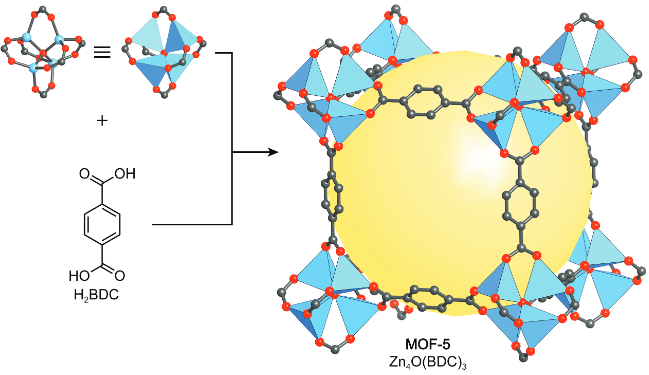
\includegraphics[width=0.7\textwidth]{fig/irmof-1.png}
	\caption[Unit cell\index{Unit cell} structure of IRMOF-1.]{Unit cell
	structure of MOF-5\index{MOF-5} or IRMOF-1\index{IRMOF-1}, one of the
	highest surface area\index{Surface area} to volume ratio among \glspl{mof},
	at \SI{2200}{\square\meter\cubic\centi\meter} and the first \gls{mof}
	studied for hydrogen storage\index{Hydrogen storage.} \parencite{Rosi2003}.}
	\label{fig:irmof-1}
\end{figure}

\section{The Problem}

The intrinsic combinatorial character of reticular chemistry, translates to
practically an infinite number of realizable structures. Currently, the
\gls{csd} contains more than \num{100000} experimentally synthesized \glspl{mof}
\parencite{siegel29} while the arrival of in silico designed \glspl{mof}
\parencite{siegel36, Rosen2021, Chung2019, chong51, DeVos2023, trillions,
Boyd_2019} has immensely expanded the available material pool. The huge size of
current and future \gls{mof} databases\index{Database} \parencite{trillions} is
both a blessing and a curse for the identification of novel materials. Blessing,
since a large number of candidate structures doesn't limit our choices and as
such, the chances to find the right material for a given problem. Curse, since
the enormous size of \glspl{mof} space makes it harder for researchers to
efficiently explore it, complicating the tracing of materials with the desired
properties. It is therefore crucial to find a way that allows us to efficiently
explore such a huge material space (see \Figure{} \ref{fig:mofs_space}). Another way
to rephrase our problem is the following: \emph{\bfseries Given a large catalog
of \glspl{mof}, is there a way to efficiently filter out the most promising ones
for the application of interest?}

As a first approach to deal with this challenge, one could, in principle
experimentally synthesize and characterize each one of the materials listed in
the given catalog. Although \emph{experimental synthesis and
characterization}\index{Experimental synthesis}\index{Experimental
characterization} is the ultimate way to assess the performance of a
material\footnote{As Richard Feynmann said: \emph{``The test of all knowledge is
experiment. Experiment is the sole judge of scientific truth''}.}, the fact that
a single laboratory study can take days or even months, renders experimental
techniques impractical.  A more efficient approach is computational
screening\index{Computational screening} based on \emph{molecular
simulations}\index{Molecular simulations}, which for years has served as the
principal tool for the discovery of high-performing \glspl{mof}
\parencite{Simon2015, chong56, Moghadam2018, chong58, chong59}. Although computational
screening dramatically accelerates the assessment of a single material compared
to experimental techniques, brute-force screening of current and upcoming
databases is considered suboptimal, given the size of the latter.

\Gls{ml}\index{Machine learning} aka \emph{data-driven\index{Data-driven}
techniques} come to the rescue when dealing with \emph{big data}\index{Big data}
and over the last years have picked up the torch from molecular simulations
regarding the screening of large databases. Given a collection of
\emph{input-output}\index{Input}\index{Output} pairs, i.e. a mathematical
representation of a material and a corresponding property, a \gls{ml}
algorithm\index{Machine learning algorithm}\footnote{Note that \gls{ml}
algorithms are not limited to solve only such kind of problems, which fall under
the umbrella of supervised learning\index{Supervised learning}. See \Section{}
\ref{subsec:paradigms} for other types of problems tackled by \gls{ml}.} seeks to
\emph{uncover the underlying structure-property relationship}. To put it in a
nutshell, a \gls{ml} algorithm ``eats'' \emph{data}\index{Data}---which may come
either from experiments, simulations or a combination of the two---and ``spits
out'' a \emph{model}\index{Model}, which can be \emph{used to sort a large
catalog of MOFs in just few seconds}. Obviously, for \gls{ml} approaches to be
effective and reliable, it is necessary that the resulting models are of high
quality.

\begin{figure}
	\centering
	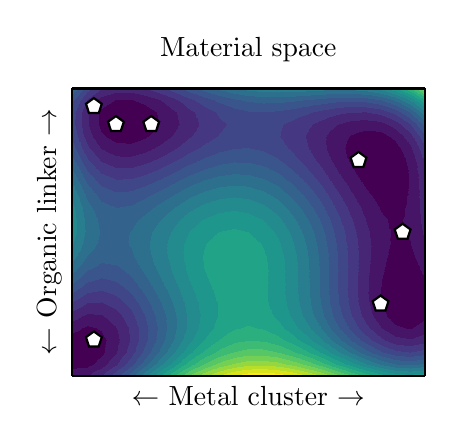
\begin{tikzpicture}
		\begin{axis}[
				%axis background/.style={fill=blue!10},
				axis lines=box, width=0.5\textwidth,
				thick, title=Material space,
				xlabel=$\leftarrow$ Metal cluster $\rightarrow$,
				ylabel=$\leftarrow$ Organic linker $\rightarrow$,
				xlabel near ticks, ylabel near ticks,
				domain=-4:4, view={0}{90}, colormap/viridis, ticks=none,
			]
			\addplot3 [contour filled={number=20}]
				{pow(x^2 + y - 11, 2) + pow(x + y^2 - 7, 2)};
			\addplot[
				only marks,
				mark options={fill=white, mark=pentagon*, scale=1.5pt,}
			] coordinates {
				(-3.5, 3.5) (-3.5, -3)
				(-3, 3) (-2.2, 3)
				(2.5, 2) (3, -2) (3.5, 0)
			};
		\end{axis}
	\end{tikzpicture}
	\caption[Material space of \acrshortpl{mof}.]{Material space\index{Material
	space} of \glspl{mof}. Each point in this space corresponds to a unique
	combination of organic linker and metal cluster, whereas the associated
	color denotes the ``score'' of material (point) for a given application.
	Finding the best material (the pentagons) for a given application, amounts
	to solving a (probably) non-convex optimization\index{Optimization}
	problem\index{Optimization problem}\index{Non-convex optimization}.}
	\label{fig:mofs_space}
\end{figure}

\section{Literature Review}
\label{sec:literature}

\emph{One of, if not the most important factor for the performance of \gls{ml}
models, is the way we select to mathematically represent materials or
molecules}. In other words, the type and amount of chemical information that is
``injected'' into these representations commonly known as
\emph{descriptors}\index{Descriptor}, can make the difference between a
high-performing and a baseline model. As such, it is of uttermost importance to
employ descriptors that provide sufficient information for the properties of
materials\index{Material} or molecules\index{Molecule} we are interested in to predict.

With regards to gas adsorption\index{Gas adsorption} in \glspl{mof}, one of the
first and most commonly used descriptors, are the so called
\emph{geometric}\index{Geometric descriptors} ones, which aim to capture the
pore environment of the framework. This type of descriptors includes textual
characteristics of \glspl{mof} such as void fraction\index{Void fraction},
gravimetric surface area\index{Gravimetric surface area} and pore limiting
diameter\index{Pore limiting diameter}. Although \gls{ml} models build with
these descriptors work particularly well at the high pressure regime
\parencite{Fernandez2013, Wu2020, Dureckova_2019}, their performance
deteriorates when adsorption takes place at low pressures\index{Pressure} or the
guest molecules exhibit non-negligible electrostatic interactions with the
framework atoms. This performance drop should be expected, since geometric
descriptors completely ignore the ``cornerstone'' of adsorption:
\emph{host-guest interactions}\index{Host-guest interactions}.

In order to improve the performance of \gls{ml} models and bypass the
limitations of geometric descriptors in the aforementioned conditions, another
type of descriptors known as \emph{energy-based} descriptors \index{Energy-based
descriptors} \parencite{chong127, Shi_2023, robust, Orhan2023}, has been
introduced. This type of descriptors supply \gls{ml} algorithms with information
regarding the energetics of adsorption, and can be used standalone or in
combination with geometric descriptors.

In one of the first works to fingerprint the energetic landscape of \glspl{mof}
\parencite{bucior}, energy histograms\index{Energy histogram} derived from the
interactions of guest molecules with the framework atoms were used to predict
hydrogen and methane uptake with remarkable accuracy. Prior to calculating the
energy histograms, a 3D grid is overlayed on the unit cell\index{Unit cell} of
the \gls{mof}. Next, at each point of the grid, the interaction between the
guest molecule with the framework atoms is calculated, producing a 3D energy
grid\index{Energy grid}. \emph{The latter is finally converted into a histogram, by
partitioning the energy values of the grid into bins of specific energy width}.
By using solely these histograms as descriptors---without including any textual
property---\textcite{bucior} trained Lasso regression
models\index{Regression}\index{Lasso regression}, for predicting:
\begin{enumerate*}
	\item \ch{H2} swing capacity\index{Swing capacity} between \SI{100}{\bar}
		and \SI{2}{\bar} at \SI{77}{\kelvin}
	\item \ch{CH4} swing capacity\index{Swing capacity} between \SI{65}{\bar}
		and \SI{5.8}{\bar} at \SI{298}{\kelvin}
\end{enumerate*}.
The resulting models were extremely accurate, achieving a \gls{mae}\index{Mean
absolute error} of \SI{2.3}{\gram\per\liter} and
\SI{12.9}{\cubic\centi\meter\per\cubic\centi\meter} for \ch{H2} and \ch{CH4},
respectively, tested on the hMOFs\index{hMOFs database} database
\parencite{siegel36}.

In another work \parencite{generic}, a set of descriptors based on the average
interaction between fictitious probe particles\index{Probe particle} and the
framework atoms was introduced. Two different types of probe particles were
proposed:
\begin{enumerate*}
	\item Vprobe particles, which account for the van der Waals
		interactions\index{Van der Waals interactions}
	\item Dprobe particles, which are neutrally charged electric dipoles and
		account for the electrostatic interactions
\end{enumerate*}.
Each of these fictitious probe particles is randomly inserted at different
positions of the unit cell\index{Unit cell}, and the interaction energy between
the probe and the framework atoms is calculated. \emph{The interaction energies at the
different positions are averaged out, producing an energetic
fingerprint\index{Energetic fingerprint} of the material}. These fingerprints in
combination with six geometric descriptors formed the input for the
\gls{rf}\index{Random forest} algorithm, which was trained to predict gas
uptake\index{Gas uptake} for a plethora of guest molecules\index{Guest molecule}
and thermodynamic conditions\index{Thermodynamic conditions}, on the
\gls{core}\index{CoRE MOF database} \gls{mof} database \parencite{chong47}. The
\gls{ml} models achieved impressive performance, showing an $R^2$  value (see
\Section{} \ref{sec:ml_details} for a definition) of:
\begin{enumerate*}
	\item \num{0.874} for \ch{H2} uptake at \SI{77}{\kelvin} and \SI{2}{\bar}
	\item \num{0.889} for \ch{CH4} uptake at \SI{298}{\kelvin} and
		\SI{5.8}{\bar}
\end{enumerate*}.
A highlight of this work was the exceptional performance of the \gls{ml} model
with regards to \ch{CO2} uptake at \SI{300}{\kelvin} and \SI{0.1}{\bar},
achieving an $R^2$ score of \num{0.832}. At the same conditions, the \gls{ml}
model trained with geometric descriptors only achieved an $R^2$ score of
\num{0.507}. That is, the ``injection'' of energetic information resulted in
\SI{60}{\percent} increase in accuracy.

\section{Thesis Statement}

In the aforedescribed works, a general pattern can be recognized with regards to
the building of the \gls{ml} models. Starting from the \gls{pes}\index{Potential
energy surface} or an approximation thereof, energetic fingerprints are manually
handcrafted based on some heuristic, and these fingerprints are then used to
train a \gls{ml} algorithm. However, a lot of information has been lost during
the conversion of the \gls{pes} into fingerprints, as a 3D object is converted
into an 1D object.  \emph{Since gas adsorption comes down to the \gls{pes}, it
is reasonable to question whether one can use the \gls{pes} itself as
descriptor}. By doing this:
\begin{enumerate*}
	\item The information content that goes into a \gls{ml} algorithm is increased
	\item The computational cost\index{Computational cost} remains the same relative
		to the previously described works
	\item It is no longer necessary to manually handcraft fingerprints
\end{enumerate*}.

\emph{In this thesis, \textbf{a generalized framework to predict gas adsorption
properties is proposed, using the \gls{pes} as raw input}. Since the latter captures
both the host-guest interactions and the geometry of the pore, i.e. the factors
that mainly determine gas uptake in the low and high pressure regime
\parencite{concepts}, respectively, it can be regarded as the perfect input. In
order to be machine understandable the \gls{pes} is first voxelized---the
voxelized \gls{pes} is essentially a 3D energy image\index{Energy image} where
each 3D pixel aka voxel, is colorized by energy---and then, it is processed by a
3D \acrlong{cnn}, known for its ability to process image-like data}. The proposed
scheme is schematically presented in \Figure{} \ref{fig:approach}.

\begin{figure}
	\centering
	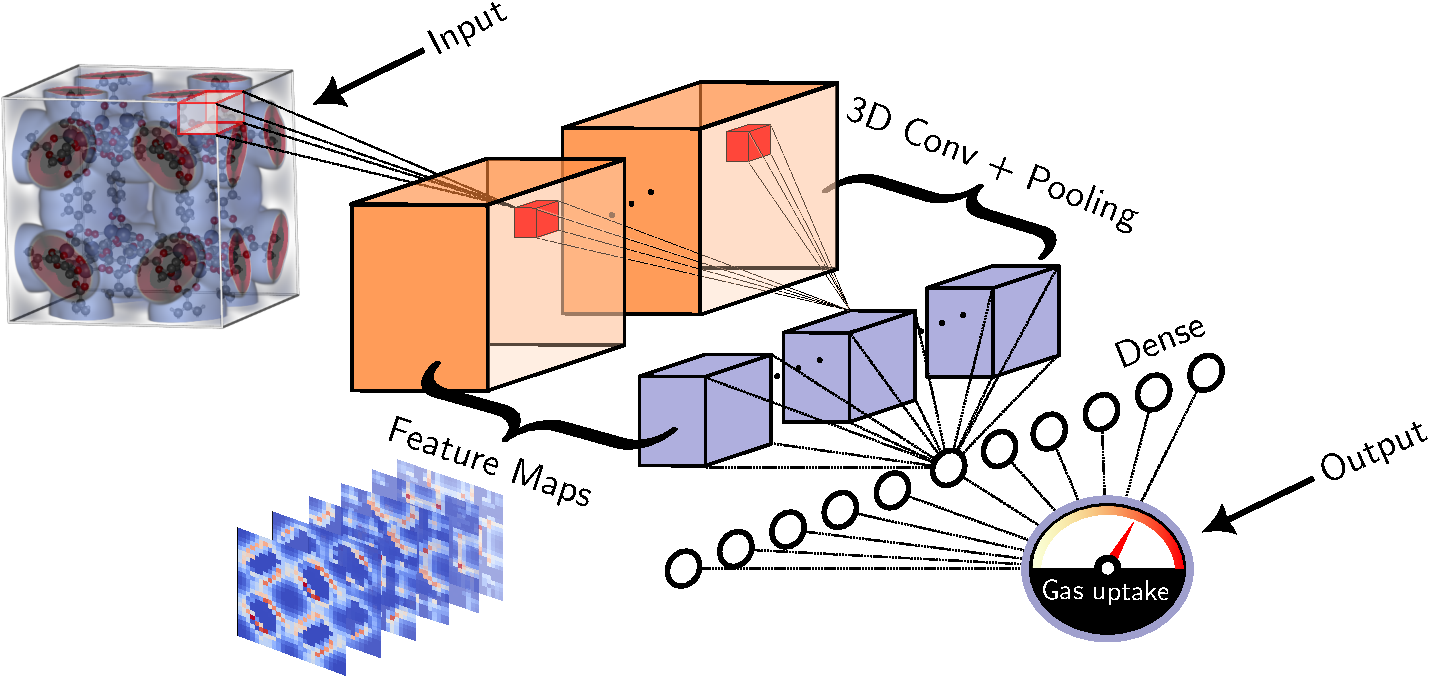
\includegraphics[width=\textwidth]{fig/approach.pdf}
	\caption[Generalized framework to predict gas adsorption
	properties.]{Proposed scheme to predict gas adsorption properties, starting
	from the \gls{pes} as raw input. A 3D \gls{cnn} extracts its
	features\index{Feature} from the \gls{pes}, and then uses them to predict
	the adsorption property of interest. The IRMOF-1 structure and PES were
	visualized with the iRASPA software \parencite{Dubbeldam2018}.}
	\label{fig:approach}
\end{figure}
